Electron fakes originate from three main sources: heavy-flavor jets, light-flavor jets, and $\gamma$ conversions. Each source has a different probability of being mis-identified as a prompt electron so naturally we would like to perform a fake factor calculation like what was done with the muon fakes. However, this is quite difficult as it is almost impossible to separate fake electrons originating from $Z+$jets and those from $Z\gamma$. Therefore, a scale factor method was developed, which essentially defines three distinct CR's that are enriched in each category of fake electrons, and then a normalization factor is calculated using the ratio of data ID events to MC simulation anti-ID events, which is then used to scale the corresponding MC samples in the SR\@.

The selections for the electron CR's are summarized in Table~\ref{tab:wh_electron_id_antiid_selection}. The CR's are designed such that they are in a phase space dominated by one of the three sources of fake electrons. The first CR is referred to as $\mathrm{CR}^{\mu^{+}\mu^{-} e}_{\gamma~\mathrm{conv.}}$, and is designed to target events where the fake electron originates from $\gamma$ conversions by selecting $Z$-boson events with a FSR photon where the $Z \to \mu^+\mu^-$ process. The second CR, $\mathrm{CR}^{\mu^{\pm}\mu^{\mp}e}_{Z+\mathrm{jets}}$, is designed to pick out events with light-flavor jet fakes from $Z+$jets where the $Z$ boson decays to two opposite sign muons. The last CR, $\mathrm{CR}^{e^{\pm}\mu^{\mp}e^{\pm}}_{t\bar{t}}$, mainly selects heavy-flavor jet fakes originating from $t\bar{t} \to W^{\pm}W^{\mp}b\bar{b}$ decays with prompt, opposite sign, $e\mu$ pairs originating from the two $W$ bosons decaying leptonically, and an additional electron mis-identified from $b$-quark hadronization. The two electrons are selected to be same sign, ensuring that the muon is uniquely charged and prompt, and one of the electrons is fake. The fake electron is considered to be the sub-leading electron in the ID region for similar reasons as given in the previous section, while the anti-ID electron is the fake electron in the anti-ID region.

\begin{table}[htp]
  \centering
  \begin{tabular}{l|l}
    \hline
    \textbf{Control Regions} & \textbf{Definitions} \\
    \hline
    \hline
    \multirow{6}{*}{Common selections for $\mu^{\pm}\mu^{\mp}e$ CR's} 
      & ID lepton matched to single lepton triggers \\
      & All lepton $\pt > 15$ GeV \\
      & $N_{b_{\mathrm{jets}}} = 0$ \\
      & $m^{\mathrm{min}}_{\mathrm{osll}} > 12$ GeV \\
      & $\metsig < 2.4$ \\
      & $m_{\mathrm{T}} < 40$ GeV \\
      \hline
    \multirow{2}{*}{$\mathrm{CR}^{\mu^{\pm}\mu^{\mp} e}_{\gamma~\mathrm{conv.}}$} & 40 GeV $< m_{\mu\mu} <$ 80 GeV \\
     & $|m_{\ell\ell\ell} - m_{Z}| < 10$ GeV \\
    \hline
    \multirow{2}{*}{$\mathrm{CR}^{\mu^{\pm}\mu^{\mp} e}_{Z+\mathrm{jets}}$} & 80 GeV $< m_{\mu\mu} < 100$ GeV \\
    & $m_{\ell\ell\ell} < 200$ GeV \\
    \hline
    \multirow{3}{*}{$\mathrm{CR}^{e^{\pm}\mu^{\mp}e^{\pm}}_{t\bar{t}}$} & ID lepton matched to single lepton triggers \\
    & All lepton $\pt > 15$ GeV \\
    & $N_{b_{\mathrm{jets}}} = 1$ \\
    \hline
  \end{tabular}
  \caption{Control region definitions used in calculating the electron scale factors. The anti-ID version is obtained by requiring the presence of an anti-ID electron as defined in Table~\ref{tab:wh_id_antiid_selection}.}\label{tab:wh_electron_id_antiid_selection}
\end{table}

Figure~\ref{fig:VH_electron_id_crs} shows the electron \pt{} distributions in the ID and anti-ID CR's previously mentioned. Different from the muon fake factor method, the scale factor is measured in the three following \pt{} bins: $15 < \pt < 20$ GeV, $20 < \pt < 30$ GeV, and $\pt > 30$ GeV. Note that the data in the anti-ID CR is not directly used in this method, so no relevance should be attached to the data-MC comparison in the CRs.

\begin{figure}[htp]
  \centering
  \subfloat[$\gamma$ Conversion ID CR]{
    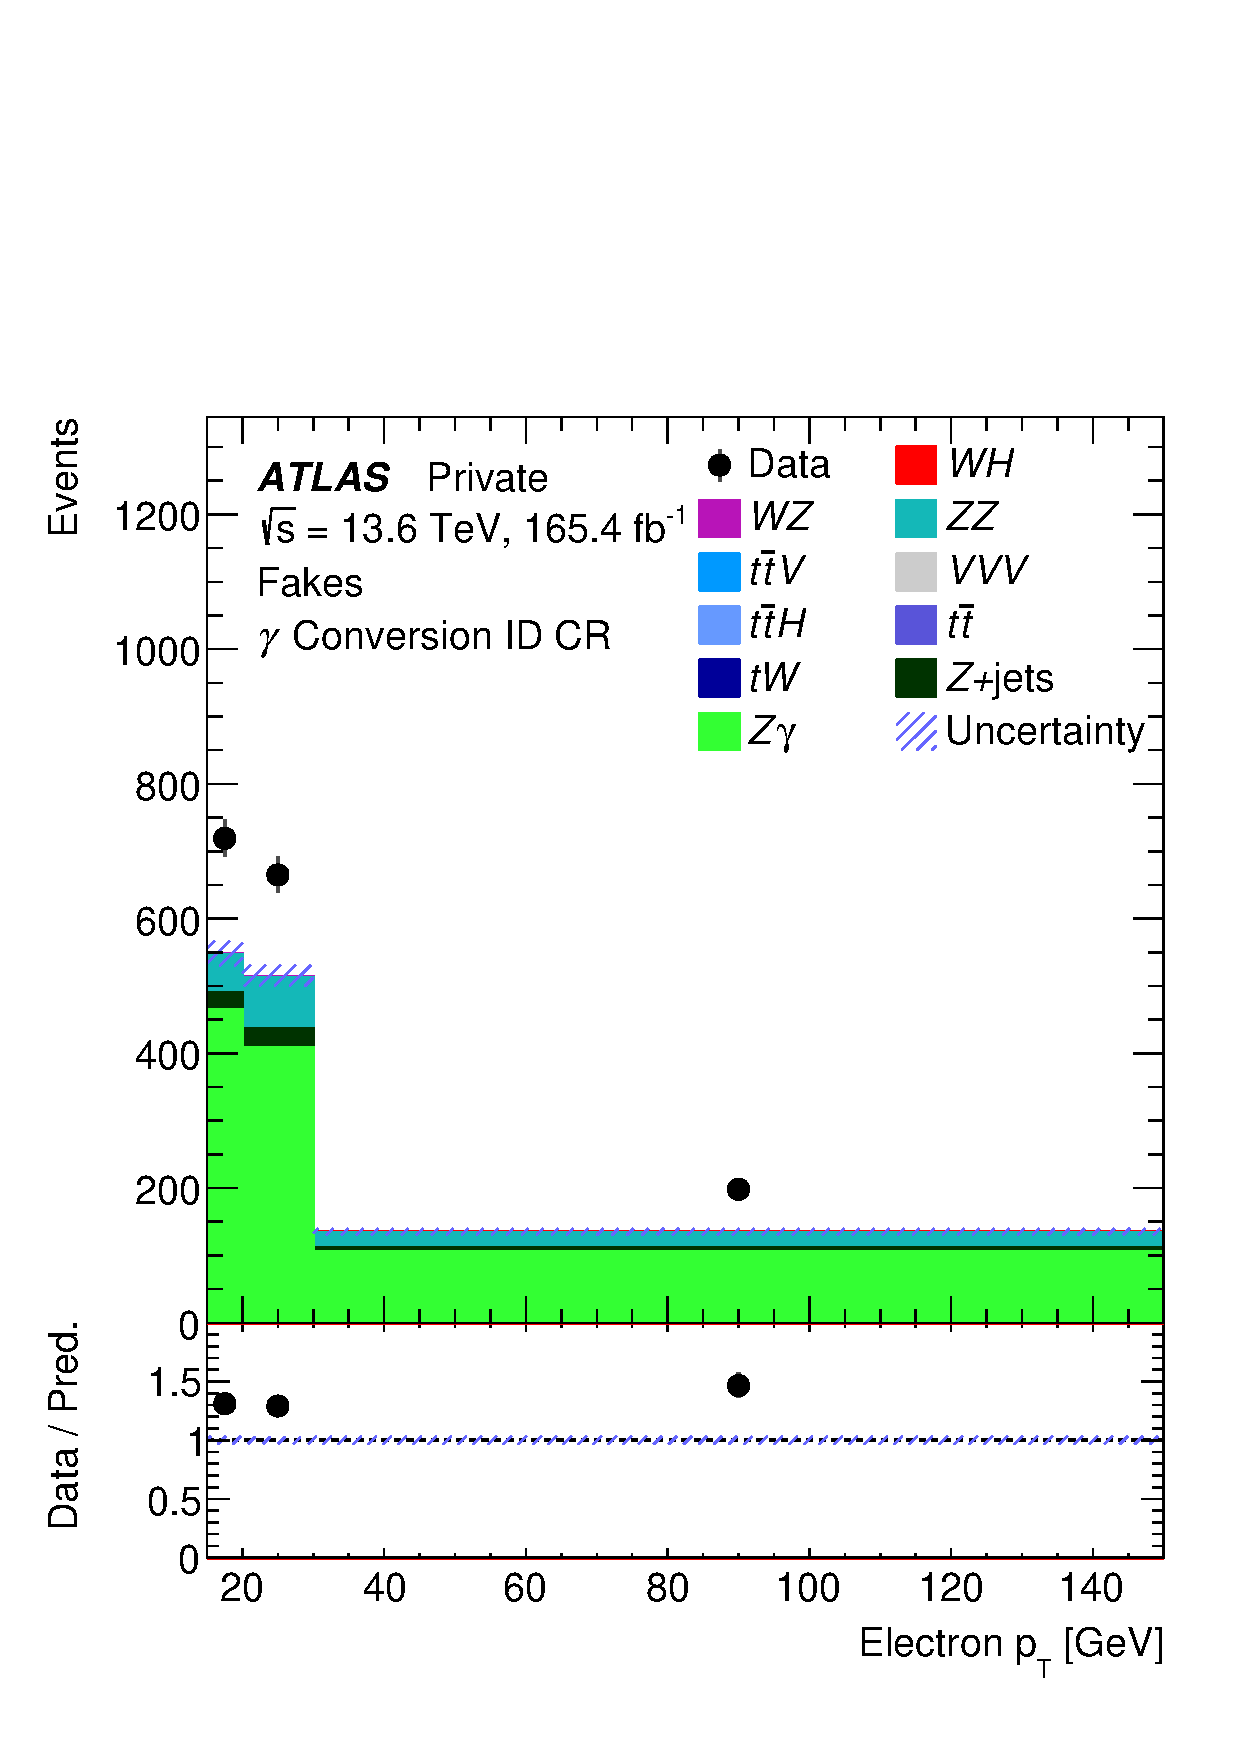
\includegraphics[width=0.34\textwidth]{figures/VH/VH_gamma_conv_id_cr.pdf}\label{fig:VH_electron_id_cr_gammaconv}
  }
  \subfloat[$\gamma$ Conversion anti-ID CR]{
    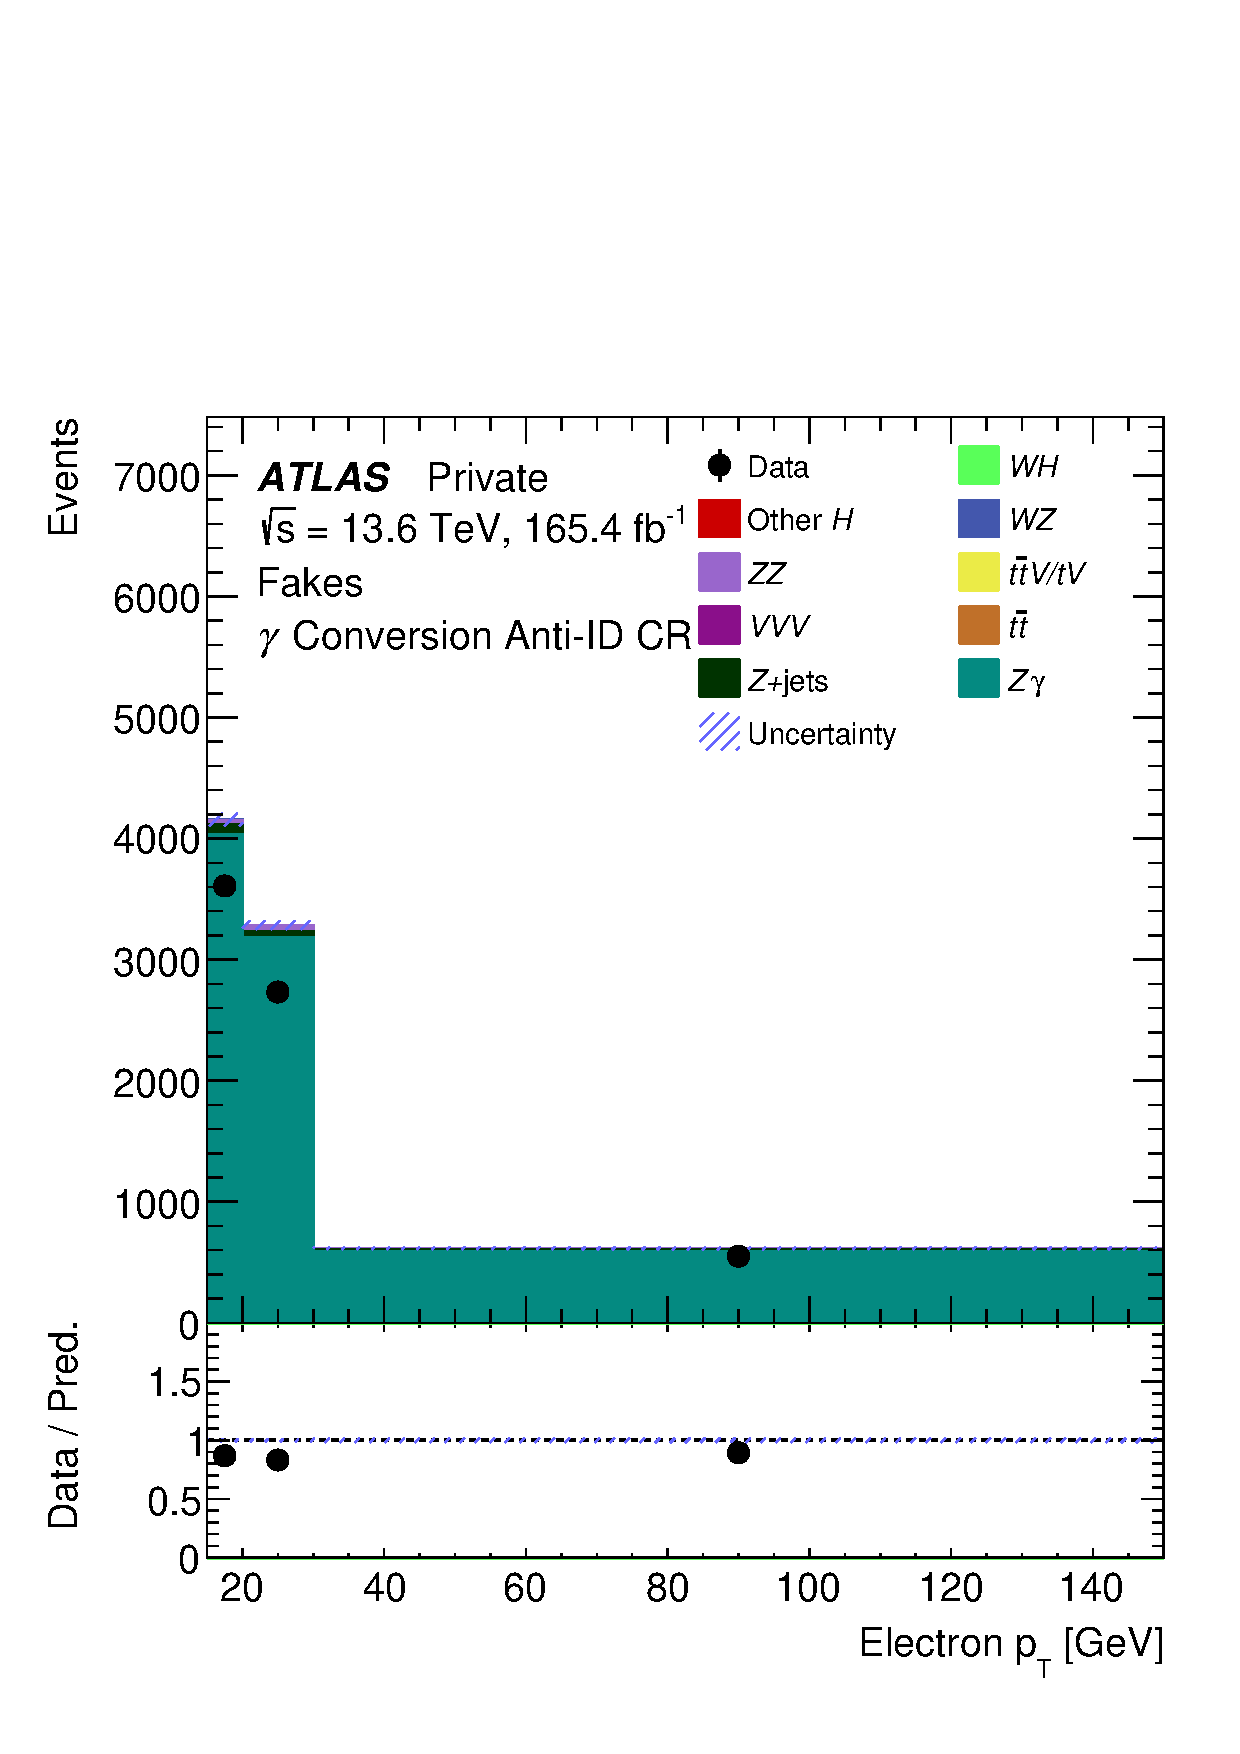
\includegraphics[width=0.34\textwidth]{figures/VH/VH_gamma_conv_aid_cr.pdf}\label{fig:VH_electron_antiid_cr_gammaconv}
  }
  \hfill
  \subfloat[Light Flavor ID CR]{
    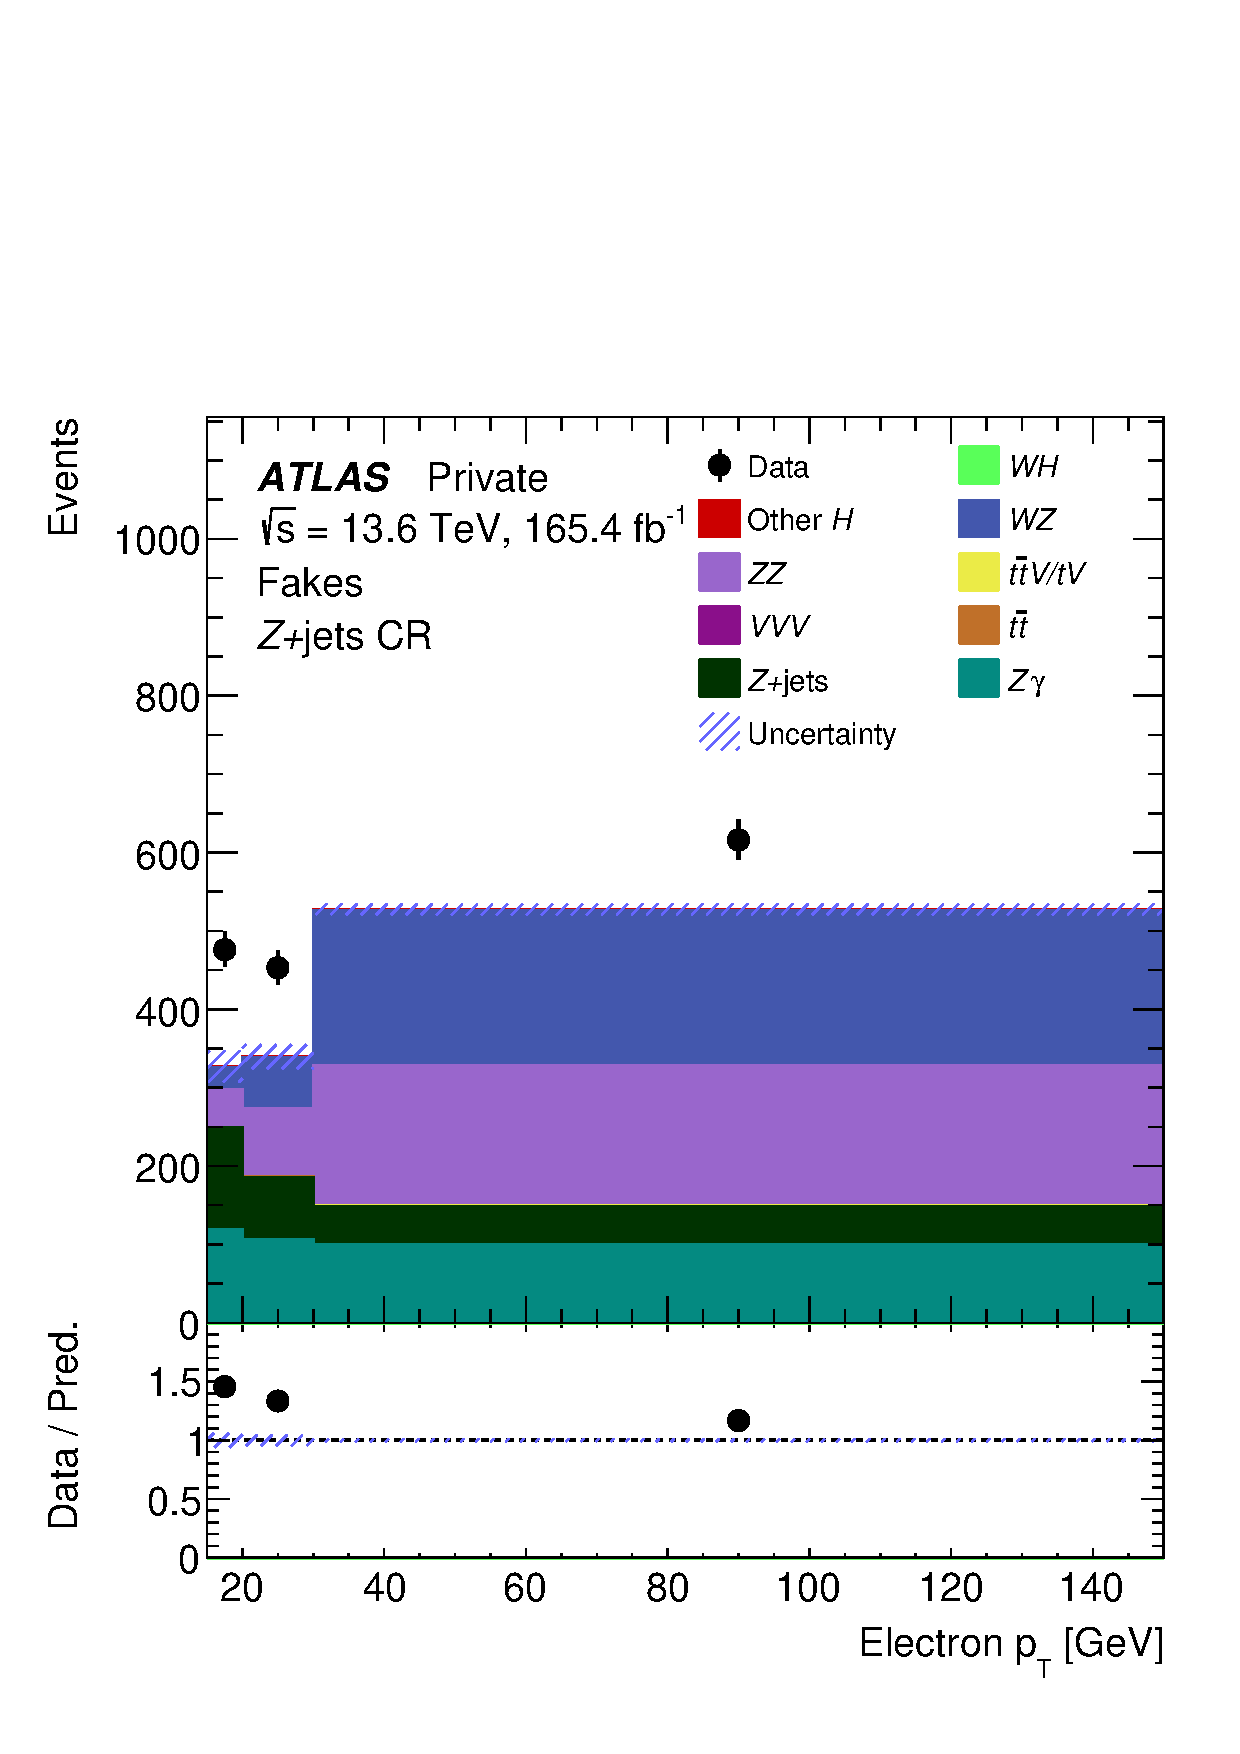
\includegraphics[width=0.34\textwidth]{figures/VH/VH_light_flavor_id_cr.pdf}\label{fig:VH_electron_id_cr_zjets}
  }
  \subfloat[Light Flavor anti-ID CR]{
    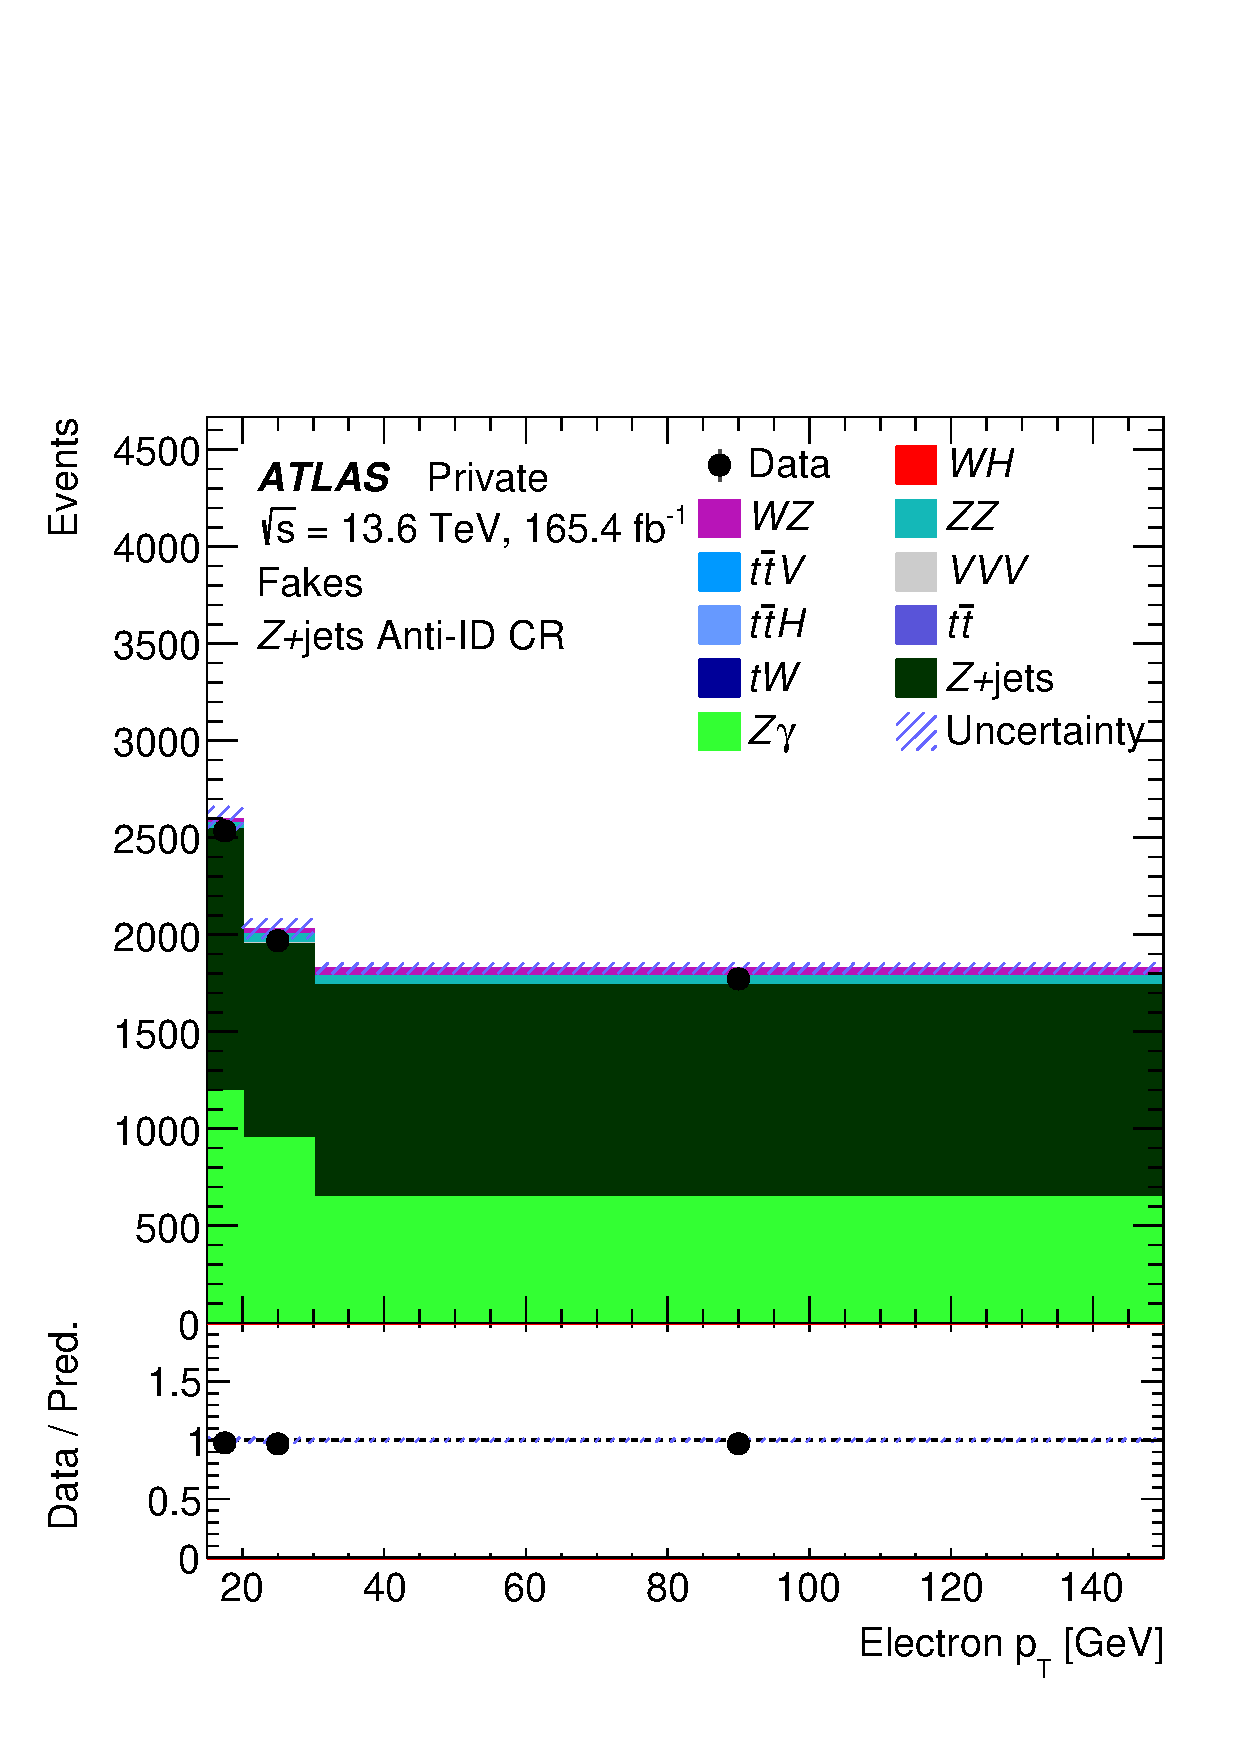
\includegraphics[width=0.34\textwidth]{figures/VH/VH_light_flavor_aid_cr.pdf}\label{fig:VH_electron_antiid_cr_zjets}
  }
  \hfill
  \subfloat[Heavy Flavor ID CR]{
    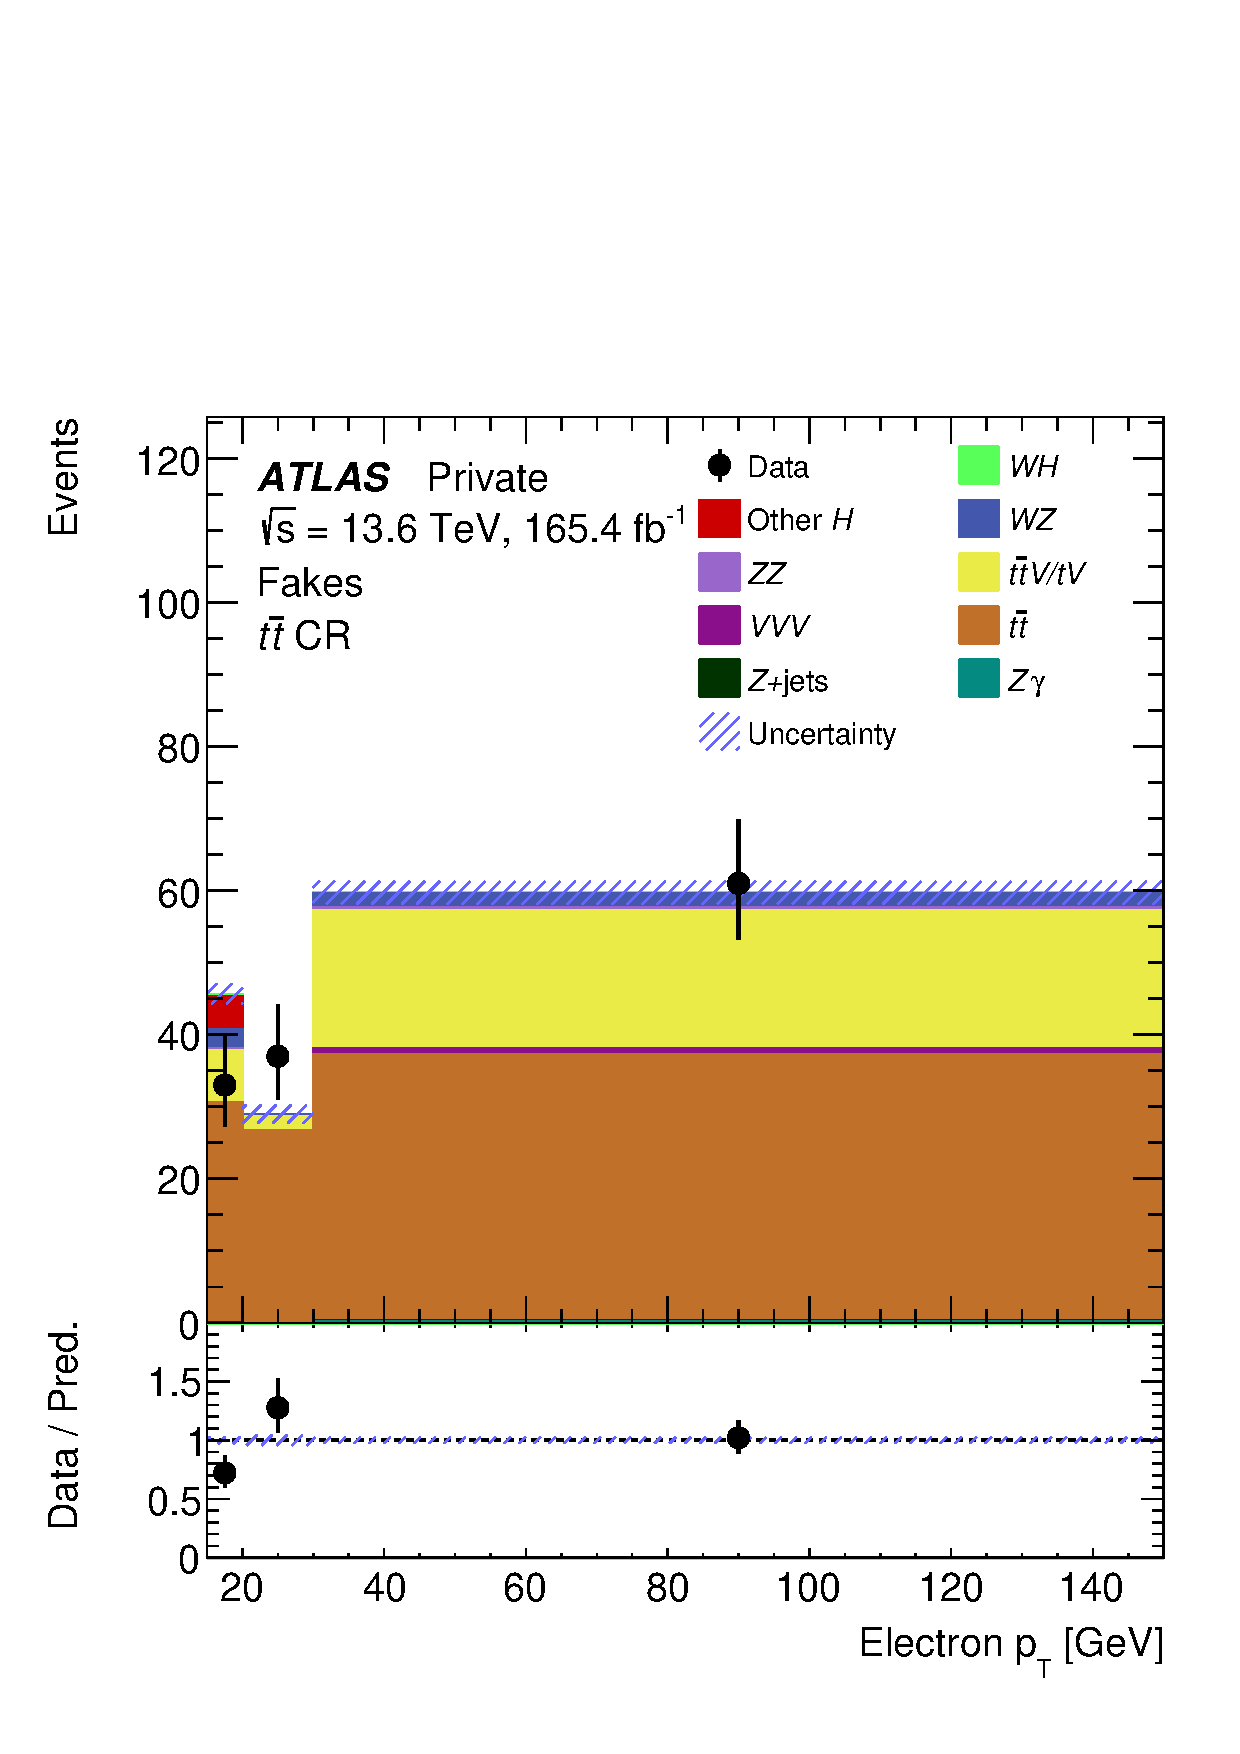
\includegraphics[width=0.34\textwidth]{figures/VH/VH_heavy_flavor_id_cr.pdf}\label{fig:VH_electron_id_cr_ttbar}
  }
  \subfloat[Heavy Flavor anti-ID CR]{
    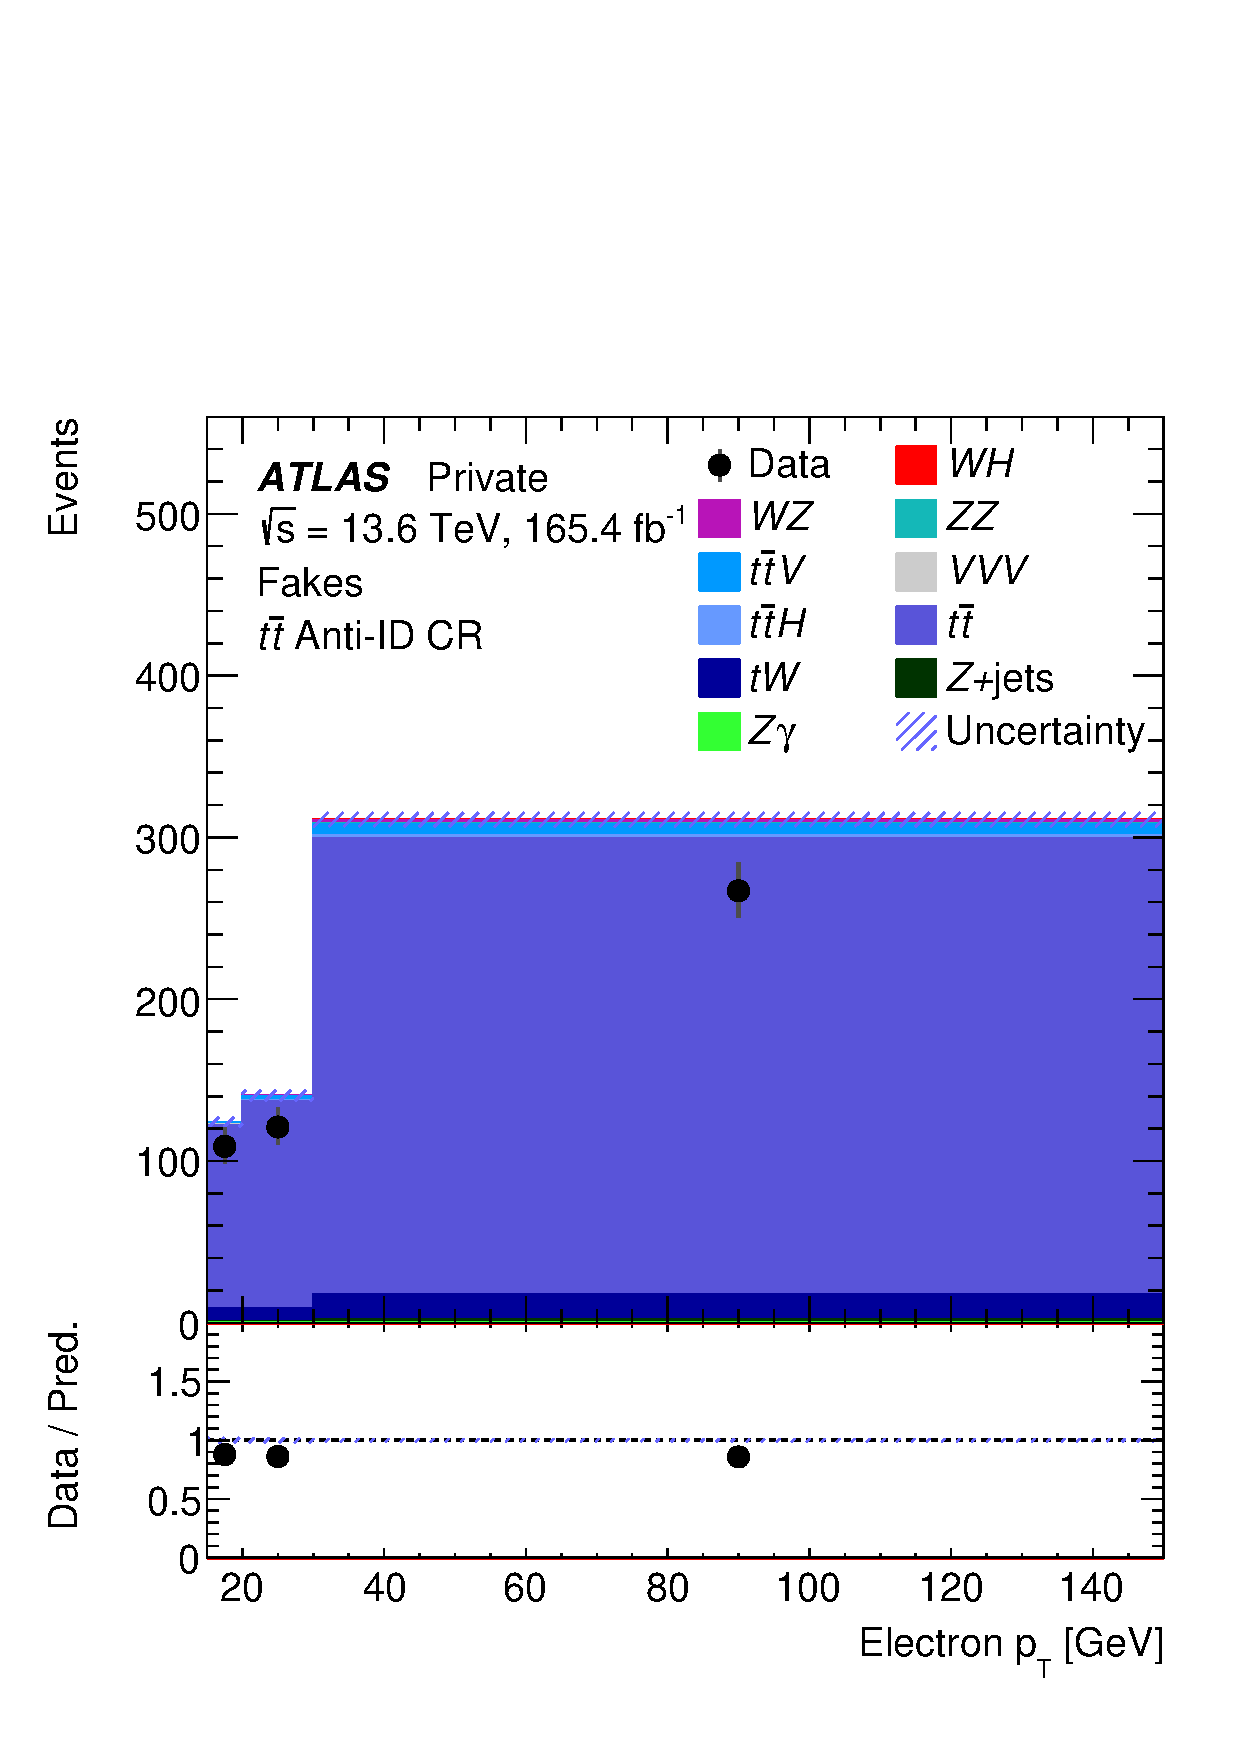
\includegraphics[width=0.34\textwidth]{figures/VH/VH_heavy_flavor_aid_cr.pdf}\label{fig:VH_electron_antiid_cr_ttbar}
  }
  \caption{Distributions of the electron \pt{} in the ID and anti-ID CR's used for the electron scale factor calculation. The $\gamma$ conversion CR is shown in (a) and (b), the light flavor CR in (c) and (d), and the heavy flavor CR in (e) and (f).}\label{fig:VH_electron_id_crs}
\end{figure}

The final CR used for obtaining the SR estimate is identical to the SR except requiring one anti-ID electron. This method assumes that for a given pair of ID and anti-ID CRs targeting background i, the follow equation holds for each \pt{} bin:
\begin{equation}\label{eq:vh_wh_electron_f}
  \sum_{i}(N^{\mathrm{ID}, i}_{\mathrm{data}} + \sum_{j}N^{\mathrm{ID}, i}_{\mathrm{prompt}, j}) = \sum_{i}\sum_{j}SF_{j} \cdot N^{\mathrm{anti-ID}, i}_{\mathrm{MC}, j}, 
\end{equation}
where $j$ corresponds to one of the prompt backgrounds $WZ$, $ZZ$, $t\bar{t}V$, $t\bar{t}H$ and $VVV$ that are estimated from MC simulation, and MC,j refers to the contribution of fake background of type $j$, either $Z+$jets, $Z\gamma$, or $t\bar{t}$, and $SF_j$ is the scale factor for that background type. Unlike muons, an isolation requirement is applied to our anti-ID electrons, thus it is not necessary to correct their \pt{} as done for the latter.

For each \pt{} bin, Equation~\ref{eq:vh_wh_electron_f} gives a system of three equations with three variables and can be directly solved. 

Scale factors are extracted similarly to the muon fake factor method, where a likelihood function $\mathcal{L}(\vec{SF})$ is defined as a product of two probability distribution functions as seen in Equation~\ref{eq:vh_wh_electron_likelihood}:
\begin{equation}
  \mathcal{L}(\vec{SF}) = \prod_{ij}\mathrm{Poisson}(N_{ij}^{\mathrm{ID, data}}; N_{ij}^{\mathrm{ID, estimated}}(\vec{\theta})) \cdot \prod_{k}\mathrm{Gaussian}(\theta_{k}; \tilde{\theta_{k}}, \Delta{\theta_{k}}),
\end{equation}\label{eq:vh_wh_electron_likelihood}
where
\begin{itemize}
  \item $N_{ij}^{\mathrm{ID, data}}$ is the data yield in the ID CR for process $j$ in \pt{} bin $i$,
  \item $N_{ij}^{\mathrm{ID, estimated}}(\vec{\theta}) = N_{ij}^{\mathrm{ID, prompt}}(\vec{\theta}) + \sum_{f}SF^{i}_{f} \cdot N_{ij}^{\mathrm{anti-ID, fake f}}$ is the sum of the prompt lepton background yield in the ID CR $j$ and the fake lepton background yield in the anti-ID CR $j$ with the scale factor for that \pt{} bin,
  \item $N_{ij}^{\mathrm{ID, prompt}}(\vec{\theta}) = \sum_{k}N_{ij}^{\mathrm{ID, prompt k}} \cdot \theta_{k}$, is the sum of the yield with normalization factor $\theta_{k}$ of each prompt process $k$ in the ID CR $j$ and \pt{} bin $i$, with $k = WZ, ZZ, VVV, t\bar{t}V, VH$, and $t\bar{t}H$.
\end{itemize}
The first term is used to extract scale factor $j$, by modeling the event yield in each \pt{} bin $i$ in the ID scale factor CR\@. The second term is a Gaussian term used to constrain the normalization of prompt lepton background $k$ via a set ($\vec{\theta}_{k}$) of NPs ($\theta_{k}$). The mean $\tilde{\theta}_{k}$ is set to 1.0 and the standard deviation $\Delta{\theta_{k}}$ is equal to $\frac{\Delta_{\sigma_{k}}}{\sigma_{k}}$ which is the relative uncertainty in the cross section of process $k$. The normalizations of the dominant prompt lepton processes are constrained using their relative cross sections uncertainties: $\frac{\Delta\sigma_{t\bar{t}V}}{\sigma_{t\bar{t}V}}$ = 13\%~\cite{ttVNLOTwiki}, $\frac{\Delta\sigma_{t\bar{t}H}}{\sigma_{t\bar{t}H}}$ = 10\%~\cite{CERNYR4Twiki}, $\frac{\Delta\sigma_{WZ}}{\sigma_{WZ}}$ = 5\%~\cite{STDM-2018-03}, $\frac{\Delta\sigma_{ZZ}}{\sigma_{ZZ}}$ = 6.5\%~\cite{ATLAS:2023dew}, and $\frac{\Delta\sigma_{VVV}}{\sigma_{VVV}}$ = 24\%~\cite{STDM-2019-09,ATLAS:2024nab}. The normalization factor for the $tZ$ process is set to 1.0.

As with the muon fake factors, we minimize the negative log-likelihood function $\mathcal{L}(\vec{SF})$ to extract the scale factors for each \pt{} bin. The resulting MC- and data-driven scale factors are shown in Tables~\ref{tab:vh_wh_electron_scale_factors_mc} and~\ref{tab:vh_wh_electron_scale_factors_dd}, respectively.

\begin{table}[htb]
  \centering
  \begin{tabular}{c|ccc}
  \hline
  & $15 < \pt < 20$~GeV & $20 < \pt <3 0$~GeV & $\pt > 30$~GeV \\
  \hline
  $Z\gamma$ & $0.12 \pm 0.01$ & $0.12 \pm 0.01$ & $0.16 \pm 0.03$ \\
  $Z+$jets & $0.09 \pm 0.01$ & $0.12 \pm 0.01$ & $0.11 \pm 0.03$ \\
  $t\bar{t}$ & $0.22 \pm 0.07$ & $0.17 \pm 0.06$ & $0.14 \pm 0.05$ \\
  \hline
  \end{tabular}
  \caption{Electron fake scale factors calculated from MC simulation.}\label{tab:vh_wh_electron_scale_factors_mc}
\end{table}

\begin{table}[htb]
  \centering
  \begin{tabular}{c|ccc}
  \hline
  & $15 < \pt < 20$~GeV & $20 < \pt < 30$~GeV & $\pt > 30$~GeV \\
  \hline
  $Z\gamma$ & $0.15 \pm 0.01$ & $0.18 \pm 0.01$ & $0.27 \pm 0.04$ \\
  $Z+$jets & $0.15 \pm 0.01$ & $0.16 \pm 0.02$ & $0.18 \pm 0.03$ \\
  $t\bar{t}$ & $0.22 \pm 0.07$ & $0.28 \pm 0.07$ & $0.18 \pm 0.05$ \\
  \hline
  \end{tabular}
  \caption{Electron fake scale factors calculated from data.}\label{tab:vh_wh_electron_scale_factors_dd}
\end{table}

This method is validated with the same non-closure approach used in the muon fake factors, where the MC-driven scale factors are used to obtain estimates of each background in the SRs, and are then compared to the MC simulation. The resulting plots are seen in Figure~\ref{fig:vh_wh_electron_scale_factors_non_closure_plots} and their corresponding uncertainties in Table~\ref{tab:vh_wh_electron_sf_non_closure_uncertainties}. Closure is good in both SR's for $Z\gamma$ and $t\bar{t}$, while for $Z+$jets the estimated background contribution is much larger than the MC simulation prediction. Since $Z+$jets is such a small part of the total electron fake background and the fake background is a sub-leading background we are not concerned with the large non-closure uncertainty that we see. The final non-closure uncertainty used is taken from the combined \zdom{} and \zdep{} SR's.

\begin{figure}[htp]
  \centering
  \subfloat[$Z\gamma$ closure]{
    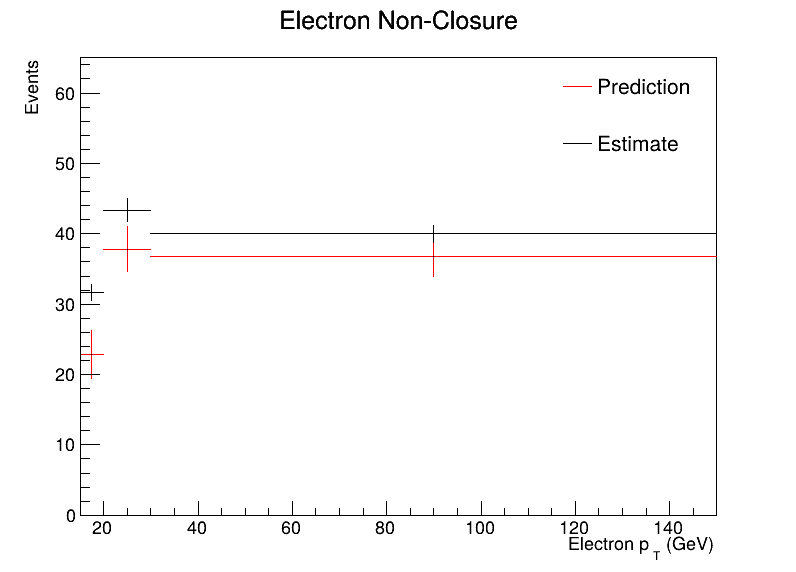
\includegraphics[width=0.49\textwidth]{figures/VH/VH_electron_sf_zgamma_nonclosure_combined.png}\label{fig:vh_wh_electron_zgamma_non_closure}
  }
  \subfloat[$Z+$jets closure]{
    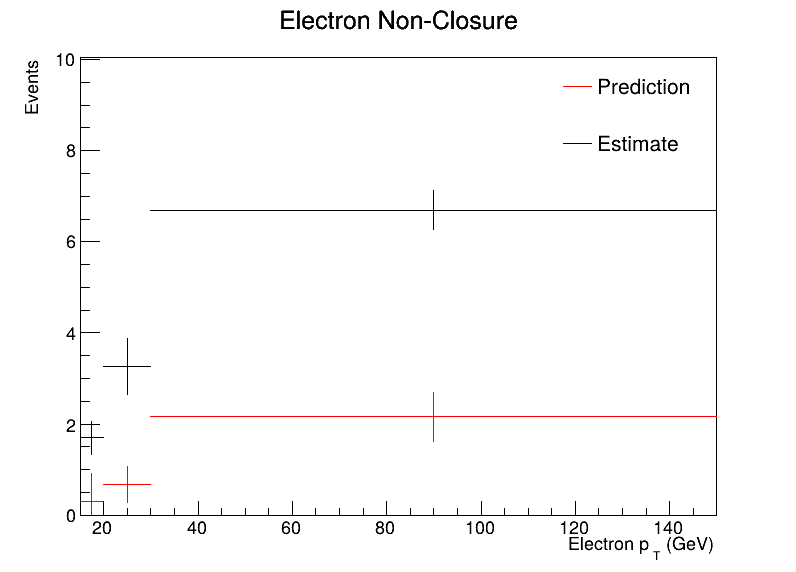
\includegraphics[width=0.49\textwidth]{figures/VH/VH_electron_sf_zjets_nonclosure_combined.png}\label{fig:vh_wh_electron_zjets_non_closure}
  }
  \hfill
  \subfloat[$t\bar{t}$ closure]{
    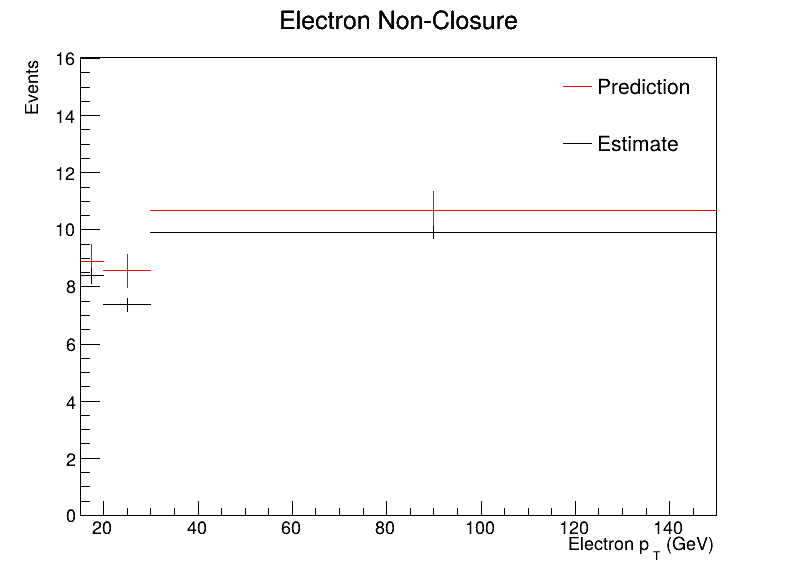
\includegraphics[width=0.49\textwidth]{figures/VH/VH_electron_sf_ttbar_nonclosure_combined.png}\label{fig:vh_wh_electron_ttbar_non_closure}
  }
  \caption{Closure test performed using the MC-driven electron fake SFs in a combined \zdep{} and \zdom{} region. The non-closure in each bin is taken as a systematic uncertainty in that bin.}\label{fig:vh_wh_electron_scale_factors_non_closure_plots}
\end{figure}

\begin{table}[htp]
  \centering
  \begin{tabular}{c|ccc}
  \hline
  & $15 < \pt < 20$~GeV & $20 < \pt < 30$~GeV & $\pt > 30$~GeV \\
  \hline
  $Z\gamma$ & $30\%$ & $15\%$ & $11\%$ \\
  $Z+$jets & $89\%$ & $80\%$ & $68\%$ \\
  $t\bar{t}$ & $9\%$ & $18\%$ & $10\%$ \\
  \hline
  \end{tabular}
  \caption{Non-closure uncertainties for the electron fake scale factors in the \wh{} analysis.}\label{tab:vh_wh_electron_sf_non_closure_uncertainties}
\end{table}
